% ============================================================================
% FROM MAKER TO CURATOR: A SCOPING REVIEW OF GENERATIVE AI IN DESIGN EDUCATION
% Enhanced Manuscript for Top-Tier Journal Submission
% Target: Design Studies / She Ji / International Journal of Art & Design Education
% ============================================================================

\documentclass[ed]{acnsart}

\setdoi{10.31812/ed.1093}
\setjournalyear{2026}
\setjournalvolume{14}
%\setjournalissue{4}
\setcounter{page}{212}


% ============================================================================
% PACKAGES
% ============================================================================

% Page layout
%\usepackage[margin=2.5cm]{geometry}
%\usepackage{setspace}
%\doublespacing

% Typography and fonts
%\usepackage[T1]{fontenc}
%\usepackage[utf8]{inputenc}
%\usepackage{mathptmx}

% Bibliography - APA style
%\usepackage[round,authoryear,sort&compress]{natbib}
%\bibliographystyle{apalike}

% Tables
\usepackage{booktabs}
\usepackage{tabularx}
\usepackage{longtable}
\usepackage{multirow}
\usepackage{array}
\newcolumntype{L}[1]{>{\raggedright\arraybackslash}p{#1}}
\newcolumntype{C}[1]{>{\centering\arraybackslash}p{#1}}
\newcolumntype{R}[1]{>{\raggedleft\arraybackslash}p{#1}}

% Graphics and Figures
\usepackage{graphicx}
\usepackage{float}

% TikZ and pgfplots for professional figures
\usepackage{tikz}
\usepackage{pgfplots}
\pgfplotsset{compat=1.18}
\usetikzlibrary{shapes.geometric, arrows.meta, positioning, calc, patterns, decorations.pathreplacing}

% Define colors for consistent visualization
\definecolor{primaryblue}{RGB}{31,119,180}
\definecolor{secondaryorange}{RGB}{255,127,14}
\definecolor{tertiarygreen}{RGB}{44,160,44}
\definecolor{quaternaryred}{RGB}{214,39,40}
\definecolor{lightgray}{RGB}{240,240,240}
\definecolor{darkgray}{RGB}{100,100,100}

% Colors and hyperlinks
\usepackage[dvipsnames]{xcolor}
%\usepackage[colorlinks=true,linkcolor=NavyBlue,citecolor=NavyBlue,urlcolor=NavyBlue]{hyperref}

% Lists
\usepackage{enumitem}

% Captions
\usepackage[labelfont=bf,font=small]{caption}
\usepackage{subcaption}

% Math
\usepackage{amsmath}
\usepackage{amssymb}

% Appendix
%\usepackage[toc,page]{appendix}

% For rotated tables if needed
\usepackage{rotating}

% Line numbers for review
%\usepackage{lineno}
% \linenumbers  % Uncomment for review

% ============================================================================
% CUSTOM COMMANDS
% ============================================================================

\newcommand{\keyterm}[1]{\textit{#1}}
\newcommand{\eg}{\textit{e.g.}}
\newcommand{\ie}{\textit{i.e.}}
\newcommand{\cf}{\textit{cf.}}
\newcommand{\etal}{\textit{et al.}}
\newcommand{\nstudies}{156}
\newcommand{\nsearched}{1800}

% ============================================================================
% DOCUMENT INFORMATION
% ============================================================================

\begin{document}

\title{From maker to curator: a scoping review of generative artificial intelligence in design higher education}

	\author{Oleksandr O. Musiienko}[
email={musyaleksandr1110@gmail.com},
url={https://kdpu.edu.ua/personal/musienko12911.html},
orcid={0000-0003-4906-8172}
] 

\address{Kryvyi Rih State Pedagogical University, 54 Universytetskyi Ave., Kryvyi Rih, 50086, Ukraine}

% ============================================================================
% BEGIN DOCUMENT
% ============================================================================



% ============================================================================
% ABSTRACT
% ============================================================================

\begin{abstract}
\noindent\textbf{Background:} The rapid proliferation of generative artificial intelligence (GenAI), particularly following ChatGPT's release in November 2022, has created unprecedented opportunities and challenges for design education. Despite intense scholarly interest, no comprehensive synthesis maps how AI is being conceptualized, implemented, and researched across design disciplines in higher education.

\noindent\textbf{Objectives:} This scoping review maps the extent, nature, and characteristics of research on generative AI in design education, examining pedagogical approaches, reported outcomes and challenges, and identifying gaps requiring future investigation.

\noindent\textbf{Eligibility criteria:} Studies addressing AI or generative AI technologies within design disciplines (architecture, fashion, graphic, product, UX/UI, interaction, or general design education) in higher education contexts, published in English between 2017--2026.

\noindent\textbf{Sources of evidence:} Web of Science Core Collection searched using 18 query combinations of design education and AI-related terms.

\noindent\textbf{Charting methods:} Data extracted using a standardized form capturing 21 variables across bibliometric, methodological, technological, and pedagogical dimensions.

\noindent\textbf{Results:} From \nsearched{} initial records, \nstudies{} studies met inclusion criteria. Publication volume increased 6.4-fold following ChatGPT's release (86.5\% post-2022). China (31.4\%) and the USA (13.5\%) dominate geographically. Research concentrates on creativity development (35.9\%), assessment (27.6\%), and curriculum design (22.4\%). Only 26.3\% employed theoretical frameworks, predominantly TPACK, design thinking, and experiential learning. Significant gaps exist in outcome reporting (66.7\% unspecified), challenge documentation (74.4\% unspecified), and methodological rigor (53.8\% lower-quality designs).

\noindent\textbf{Conclusions:} While research on generative AI in design education has surged, the field remains theoretically underdeveloped and methodologically nascent. We propose a research agenda prioritizing longitudinal studies, theoretical integration, under-researched disciplines (particularly graphic design), and ethical frameworks. The emerging paradigm shift from ``maker'' to ``curator'' demands reconceptualization of design education's foundational pedagogies.
\end{abstract}

\begin{keywords}
generative artificial intelligence \sep
design education \sep
scoping review \sep
higher education \sep
creativity \sep
design pedagogy \sep
TPACK \sep
human-AI collaboration
\end{keywords}

\maketitle


% ============================================================================
% 1. INTRODUCTION
% ============================================================================

\section{Introduction}

\subsection{The generative AI Disruption in creative education}

The global landscape of design education is navigating a period of profound structural metamorphosis, precipitated by the rapid maturation and systemic integration of generative artificial intelligence (GenAI). Within months of ChatGPT's public release in November 2022, followed by image generation tools such as DALL-E 2, Midjourney, and Stable Diffusion, educators across design fields have been compelled to fundamentally reconsider what it means to teach~-- and learn~-- design. As \citet{Fleischmann2024} observe, generative AI is ``starting to become an indispensable tool for ideation and prototyping, two fundamental skills taught in design's studio pedagogy'' \cite[p.~2]{Fleischmann2024}. Unlike previous waves of technological change, from computer-aided design in the 1980s to parametric modeling in the 2000s, generative AI does not merely augment the designer's toolkit; it intervenes directly in the cognitive and creative processes that have historically defined the discipline's core educational mission.

The scale and speed of this transformation are unprecedented. Survey data indicate that nearly 85\% of educators and 86\% of students utilized AI during the 2024--2025 academic period, yet the lack of formal training has created what practitioners describe as a ``competency gap'', where adoption velocity outpaces the development of critical literacy and ethical frameworks \cite{Pudasaini2025}. This rapid, largely ad hoc integration raises fundamental questions: If AI can generate design artifacts of professional quality, what uniquely human competencies should design curricula develop? How should assessment practices evolve when the boundary between student work and AI assistance becomes porous? What ethical frameworks should guide integration of these powerful tools?

\subsection{Design education's distinctive pedagogical context}

Design education occupies a distinctive pedagogical space that amplifies both the opportunities and challenges of AI integration. Unlike disciplines where knowledge transmission relies primarily on verbal or written forms, design education has historically privileged \keyterm{learning by doing}~-- the iterative development of design judgment through hands-on practice with materials, processes, and critique \cite{Schon1983}. The studio model, described by \citet{Shulman2005} as one of the professions' ``signature pedagogies'', creates a social and material context where students develop not only technical skills but also professional identity, critical sensibility, and what \citet{Cross2011} terms ``designerly ways of knowing''.

The design critique, or ``crit'', serves as a primary mechanism of assessment and feedback, where students present work for scrutiny by peers and instructors \cite{AbdElLatif2020}. This collaborative typology adds to critique's importance as an educational tool, fostering both explicit knowledge transmission and the development of tacit judgment that characterizes design expertise \cite{Fleischmann2025}. As \citet{Tufek2022} demonstrates, even the transition to online environments during the pandemic revealed how deeply design pedagogy depends on the physical and social affordances of studio culture.

Generative AI disrupts this model at multiple levels. At the level of skill development, AI tools can now perform tasks~-- generating alternatives, visualizing concepts, iterating on feedback~-- that previously required extensive practice to master. Research on text-to-image tools indicates that platforms like Midjourney can produce planimetric images and quality architectural visualizations, though they currently lack the ``syntactic and functional logic'' required for professional design applications \cite{FernandezMorales2024}. At the level of assessment, the ease with which AI produces polished deliverables complicates traditional evaluation methods that assumed artifacts reflected individual learning. At the level of professional identity, the repositioning of the designer from ``maker'' to ``curator'' or ``prompter'' of AI-generated content challenges long-standing conceptions of design authorship and creativity \cite{Iranmanesh2024}.

\subsection{The emerging paradigm: from pixel-pusher to art director}

Contemporary discourse increasingly frames the designer's evolving role as a transition from technical executor to creative director. As practitioners observe, ``the designer is responsible for defining the vision, orchestrating the user experience, and making the final judgment on which AI outputs align with the brand's core values'' \cite{Turchi2023}. Designers are now directors who must understand composition, hierarchy, and typography to refine the raw outputs of generative models~-- while an AI can generate aesthetically pleasing imagery, it takes human judgment to understand ``the psychology, cultural context, and emotional resonance'' that effective design requires.

This shift demands what some scholars term ``Metadesign''~-- designing the process itself. The Technological Pedagogical Content Knowledge (TPACK) framework has emerged as a prominent theoretical lens for understanding how educators might integrate AI tools effectively \cite{Lee2024, Bower2017}. Originally developed for general educational technology, TPACK emphasizes the intersection of technological knowledge, pedagogical knowledge, and content knowledge~-- a convergence particularly relevant when AI tools transform all three domains simultaneously.

Prompt engineering has emerged as a formal discipline, taught at institutions including Georgia Tech, Columbia University, and RISD \cite{MedelVera2025}. Curricula now address the ``basics of prompting'', iterative design through ``prompt chaining'', and critical evaluation of AI outputs, including guarding against ``hallucinations'' where AI produces convincing but factually incorrect content. \citet{MedelVera2025} demonstrate that semantic richness in text prompts correlates with more open-ended and expressive AI-generated images, suggesting that prompt literacy represents a genuinely new form of design competency rather than merely a technical skill.

\subsection{The need for systematic synthesis}

Despite the intensity of current discussions, understanding of how AI is actually being integrated into design education remains fragmented. Individual studies report on specific interventions, tools, or institutional responses, but no comprehensive synthesis has mapped the emerging research landscape. This gap is particularly problematic given the rapid pace of change: educators making curricular decisions need synthesized evidence, not scattered anecdotes; researchers entering the field need to understand what has been studied, what methods employed, and where gaps remain; policymakers and institutional leaders need evidence-based guidance on resource allocation, faculty development, and academic integrity policies.

Scoping reviews are particularly well-suited to this moment. Unlike systematic reviews assessing the effectiveness of specific interventions, scoping reviews aim to map the extent and nature of a research area, identify key concepts and gaps, and inform future research priorities \cite{Arksey2005, Tricco2018}. For an emerging field characterized by conceptual plurality, methodological diversity, and rapid evolution, this mapping function provides essential groundwork for more focused synthesis efforts to follow.

\subsection{Research questions}

This scoping review addresses four research questions:

\begin{enumerate}[label=\textbf{RQ\arabic*:}, leftmargin=2cm, itemsep=0.5em]
    \item What is the extent, range, and nature of research on AI and generative AI in design education?
    \item What pedagogical approaches, frameworks, and implementation strategies are being employed or proposed?
    \item What outcomes, benefits, challenges, and ethical considerations are reported in the literature?
    \item What gaps exist in the current literature, and what directions should future research prioritize?
\end{enumerate}

\subsection{Contribution and structure}

This review makes three primary contributions. First, it provides the first comprehensive map of research on generative AI in design education, synthesizing findings across design disciplines, geographic contexts, and research traditions. Second, it identifies significant gaps~-- theoretical, methodological, disciplinary, and geographic~-- that can guide future research investment. Third, it proposes a structured research agenda prioritizing the studies most needed to inform evidence-based practice.

The remainder of this paper is organized as follows. Section~\ref{sec:methods} describes the scoping review methodology, including eligibility criteria, search strategy, and data extraction procedures. Section~\ref{sec:results} presents results, beginning with study selection and characteristics, followed by thematic findings organized around the research questions. Section~\ref{sec:discussion} discusses implications, situates findings within broader theoretical and practical contexts, acknowledges limitations, and proposes future research directions. Section~\ref{sec:conclusion} concludes with key takeaways and a call to action for the design education community.

% ============================================================================
% 2. METHODS
% ============================================================================

\section{Methods}
\label{sec:methods}

\subsection{Scoping review methodology and rationale}

This study employed a scoping review methodology following the framework originally proposed by \citet{Arksey2005} and subsequently refined by \citet{Levac2010} and the Joanna Briggs Institute \cite{Peters2020}. Reporting adheres to the Preferred Reporting Items for Systematic Reviews and Meta-Analyses extension for Scoping Reviews (PRISMA-ScR) \cite{Tricco2018}.

Scoping reviews are appropriate when the aim is to map the extent and nature of research activity in a field, identify key concepts and knowledge gaps, and inform future research priorities~-- precisely the objectives of this study. Unlike systematic reviews, scoping reviews typically do not assess quality of included studies or synthesize findings into pooled effect estimates; rather, they provide comprehensive overviews of available evidence regardless of study design \cite{Munn2018}. Given the emerging, heterogeneous, and rapidly evolving nature of research on AI in design education, a scoping approach enables the breadth necessary for meaningful synthesis.

\subsection{Eligibility criteria}

Eligibility criteria were developed using the Population-Concept-Context (PCC) framework recommended for scoping reviews \cite{Peters2020}. Table~\ref{tab:inclusion} presents inclusion criteria and table~\ref{tab:exclusion} presents exclusion criteria with rationale.

\begin{table}[htbp]
\centering
\caption{Inclusion criteria based on PCC framework.}
\label{tab:inclusion}
%\small
\begin{tabularx}{\textwidth}{@{}lX@{}}
\toprule
\hfill \textbf{Criterion} & \hfil \textbf{Specification} \\
\midrule
\textbf{Population} & Students, educators, or programs in design higher education \\
\addlinespace
\textbf{Concept} & Artificial intelligence, generative AI, machine learning, deep learning, large language models, or specific AI tools (ChatGPT, DALL-E, Midjourney, Stable Diffusion, etc.) \\
\addlinespace
\textbf{Context} & Higher education settings including universities, colleges, polytechnics, and professional design programs \\
\addlinespace
\textbf{Design disciplines} & Architecture, fashion design, graphic/visual design, product/industrial design, UX/UI design, interaction design, interior design, game design, or general design education \\
\addlinespace
\textbf{Language} & English \\
\addlinespace
\textbf{Date range} & 2017--2026 \\
\addlinespace
\textbf{Publication type} & Peer-reviewed journal articles and conference papers indexed in Web of Science \\
\bottomrule
\end{tabularx}
\end{table}

\begin{table}[htbp]
\centering
\caption{Exclusion criteria with rationale.}
\label{tab:exclusion}
\small
\begin{tabularx}{\textwidth}{@{}lX@{}}
\toprule
\hfill \textbf{Criterion} & \hfil \textbf{Rationale} \\
\midrule
Non-design disciplines & Studies on AI in medical, legal, business, or engineering education without explicit design focus fall outside scope \\
\addlinespace
K-12 education only & Different pedagogical context; this review focuses on higher education \\
\addlinespace
Design practice without education & Studies on AI in professional design practice without educational component \\
\addlinespace
Technology development only & Studies developing AI systems without educational application or evaluation \\
\addlinespace
Non-English language & Practical limitation ensuring consistent analysis \\
\addlinespace
Pre-2017 publication & Predates significant advances in deep learning and generative AI \\
\addlinespace
Editorials, opinions, news & Non-peer-reviewed content lacking methodological rigor \\
\bottomrule
\end{tabularx}
\end{table}

\subsection{Information sources}

Web of Science Core Collection served as the primary database. This decision reflected: (1) comprehensive coverage of high-quality peer-reviewed research across disciplines; (2) strong indexing of design, education, and computer science journals; (3) standardized metadata facilitating systematic analysis; and (4) practical considerations of search functionality and export capabilities.

While acknowledging that additional databases (Scopus, ERIC) might capture additional relevant literature, the decision to focus on a single comprehensive database balanced thoroughness against feasibility for a single-reviewer study. This limitation is addressed in section~\ref{sec:limitations}.

\subsection{Search strategy}

The search strategy was developed iteratively, combining terms related to design education with terms related to artificial intelligence. Eighteen search queries were constructed by crossing design discipline terms with AI technology terms:
%. The complete search strategy is provided in Appendix~\ref{app:search}.
%
%\section{Complete Search Strategy}
%\label{app:search}
%
%The following 18 search queries were executed in Web of Science Core Collection in January 2026:

\begin{enumerate}[itemsep=0.2em]
	\item TS=(``architecture'' AND ``artificial intelligence'' AND ``education'')
	\item TS=(``fashion design'' AND ``artificial intelligence'')
	\item TS=(``graphic design'' AND ``artificial intelligence'' AND ``education'')
	\item TS=(``product design'' AND ``artificial intelligence'' AND ``education'')
	\item TS=(``UX design'' AND ``artificial intelligence'')
	\item TS=(``interaction design'' AND ``artificial intelligence'' AND ``education'')
	\item TS=(``design education'' AND ``artificial intelligence'')
	\item TS=(``design pedagogy'' AND ``artificial intelligence'')
	\item TS=(``design studio'' AND ``artificial intelligence'')
	\item TS=(``design education'' AND ``generative AI'')
	\item TS=(``design education'' AND ``ChatGPT'')
	\item TS=(``design education'' AND ``machine learning'')
	\item TS=(``design education'' AND ``deep learning'')
	\item TS=(``design pedagogy'' AND ``generative AI'')
	\item TS=(``architecture education'' AND ``generative AI'')
	\item TS=(``design'' AND ``higher education'' AND ``large language model'')
	\item TS=(``creative education'' AND ``artificial intelligence'')
	\item TS=(``design thinking'' AND ``artificial intelligence'' AND ``education'')
\end{enumerate}

%All searches were limited to publication years 2017--2026 and English language.



Design discipline terms included: ``architecture'', ``fashion design'', ``graphic design'', ``product design'', ``UX design'', ``interaction design'', ``design education'', ``design pedagogy'', and ``design studio''. AI technology terms included: ``artificial intelligence'', ``generative AI'', ``ChatGPT'', ``machine learning'', ``deep learning'', and ``large language model''.

Searches were conducted in January 2025, with date range limited to 2017--2026. The 2017 start date reflects significant advances in deep learning and neural networks that preceded the current generative AI era, ensuring capture of foundational work while maintaining focus on contemporary relevance.

\subsection{Selection of sources of evidence}

Source selection proceeded in two stages: (1) title and abstract screening, and (2)~full-text eligibility assessment.

In title and abstract screening, records were evaluated against inclusion and exclusion criteria based on information available in title, abstract, and keywords. Records were classified as ``Include'', ``Exclude'', or ``Uncertain''. Records classified as ``Include'' or ``Uncertain'' proceeded to full-text assessment.

In full-text assessment, eligibility of remaining records was evaluated based on detailed abstract review and available metadata. Screening was conducted by a single reviewer. While dual independent screening represents the gold standard for systematic reviews, scoping reviews conducted by single researchers are common and acceptable, particularly in emerging fields where the primary goal is mapping rather than definitive synthesis \cite{Levac2010}.

\subsection{Data charting process}

A data charting form was developed to extract relevant information from included studies. The form was piloted on an initial sample of 20 studies and refined based on emerging patterns. Twenty-one variables were extracted across four domains:

\begin{enumerate}%[leftmargin=1cm, itemsep=0.2em]
    \item \textit{Bibliometric} -- first author, publication year, title, journal/venue, DOI, country of first author affiliation.
    \item \textit{Study characteristics} -- study design, sample size, design discipline, educational level, theoretical framework.
    \item \textit{AI characteristics} -- type of AI technology, specific tools mentioned, role of AI in educational context.
    \item \textit{Pedagogical dimensions} -- focus areas, implementation context, reported outcomes, reported challenges.
\end{enumerate}

\subsection{Synthesis of results}

Results were synthesized using a combination of descriptive numerical analysis and thematic analysis. Descriptive statistics were calculated for bibliometric and study characteristics. Thematic analysis followed the approach described by \citet{Braun2006}, involving iterative coding of extracted data to identify patterns across included studies.

Findings are organized around the four research questions, with descriptive results addressing RQ1 (extent and nature), pedagogical findings addressing RQ2 (approaches and frameworks), outcome and challenge findings addressing RQ3, and gap analysis addressing RQ4.

% ============================================================================
% 3. RESULTS
% ============================================================================

\section{Results}
\label{sec:results}

\subsection{Selection of sources of evidence}

Figure~\ref{fig:prisma} presents the PRISMA flow diagram summarizing the study selection process. The search of Web of Science yielded \nsearched{} records. After removing 50 duplicates, 1,750 unique records were screened at the title and abstract level.

\begin{figure}[htbp]
\centering
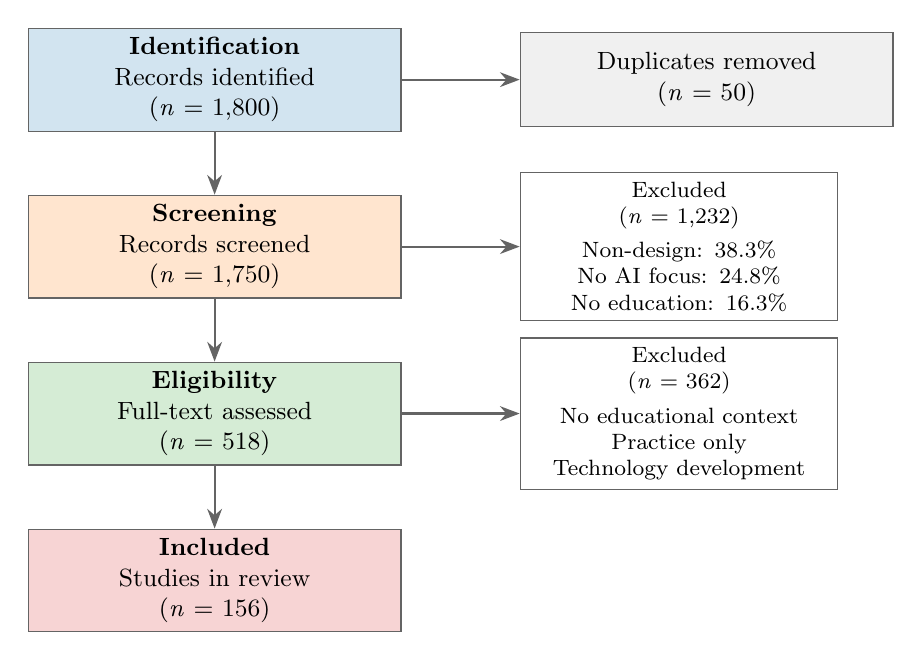
\begin{tikzpicture}[
    node distance=0.8cm,
    box/.style={rectangle, draw=darkgray, fill=lightgray, text width=4.5cm, minimum height=1.2cm, align=center, font=\small},
    exclusion/.style={rectangle, draw=darkgray, text width=3.8cm, minimum height=0.9cm, align=center, font=\footnotesize},
    arrow/.style={-{Stealth[length=2.5mm]}, thick, darkgray}
]

% Identification
\node[box, fill=primaryblue!20] (id) {\textbf{Identification}\\Records identified\\(\textit{n} = 1,800)};

% Duplicates
\node[box, right=1.5cm of id] (dup) {Duplicates removed\\(\textit{n} = 50)};
\draw[arrow] (id) -- (dup);

% Screening
\node[box, fill=secondaryorange!20, below=of id] (screen) {\textbf{Screening}\\Records screened\\(\textit{n} = 1,750)};
\draw[arrow] (id) -- (screen);

% Excluded at screening
\node[exclusion, right=1.5cm of screen] (excl1) {Excluded\\(\textit{n} = 1,232)\\[0.1cm]\footnotesize Non-design: 38.3\%\\No AI focus: 24.8\%\\No education: 16.3\%};
\draw[arrow] (screen) -- (excl1);

% Eligibility
\node[box, fill=tertiarygreen!20, below=of screen] (elig) {\textbf{Eligibility}\\Full-text assessed\\(\textit{n} = 518)};
\draw[arrow] (screen) -- (elig);

% Excluded at eligibility
\node[exclusion, right=1.5cm of elig] (excl2) {Excluded\\(\textit{n} = 362)\\[0.1cm]\footnotesize No educational context\\Practice only\\Technology development};
\draw[arrow] (elig) -- (excl2);

% Included
\node[box, fill=quaternaryred!20, below=of elig] (incl) {\textbf{Included}\\Studies in review\\(\textit{n} = 156)};
\draw[arrow] (elig) -- (incl);

\end{tikzpicture}
\caption{PRISMA flow diagram of study selection process.}
\label{fig:prisma}
\end{figure}

Of the 1,750 screened records, 1,232 (70.4\%) were excluded at title/abstract stage. Primary exclusion reasons were: non-design discipline focus (38.3\%), lack of AI/technology focus (24.8\%), lack of educational focus (16.3\%), and other reasons including non-English language and publication type (20.6\%).

The remaining 518 records proceeded to eligibility assessment. Of these, 362 (69.9\%) were excluded, predominantly for lacking explicit educational context (\ie, studies on AI in design practice without pedagogical focus). The final sample comprised \nstudies{} studies.

\subsection{Characteristics of included sources}

\subsubsection{Temporal distribution}

The temporal distribution of included studies reveals dramatic growth in research activity, with 86.5\% of studies published after ChatGPT's release in November 2022. Figure~\ref{fig:temporal} visualizes this distribution.

%\begin{figure}[htbp]
%\centering
%\begin{tikzpicture}
%\begin{axis}[
%    ybar,
%    width=0.9\textwidth,
%    height=7cm,
%    bar width=0.6cm,
%    ylabel={Number of studies},
%    xlabel={Publication year},
%    symbolic x coords={2018, 2019, 2020, 2021, 2022, 2023, 2024, 2025, 2026},
%    xtick=data,
%    ymin=0,
%    ymax=100,
%    ytick={0, 20, 40, 60, 80, 100},
%    nodes near coords,
%    nodes near coords align={vertical},
%    every node near coord/.append style={font=\footnotesize},
%    legend style={at={(0.02,0.98)}, anchor=north west, font=\small},
%    area legend,
%    enlarge x limits=0.1,
%]
%
%% Pre-ChatGPT (light color)
%\addplot[fill=primaryblue!40, draw=primaryblue] coordinates {
%    (2018, 2)
%    (2019, 2)
%    (2020, 4)
%    (2021, 9)
%    (2022, 4)
%};
%
%% Post-ChatGPT (dark color)
%\addplot[fill=quaternaryred!70, draw=quaternaryred] coordinates {
%    (2023, 9)
%    (2024, 36)
%    (2025, 87)
%    (2026, 3)
%};
%
%\legend{Pre-ChatGPT (\textit{n}=21), Post-ChatGPT (\textit{n}=135)}
%
%% Add annotation for ChatGPT release
%\draw[dashed, thick, darkgray] (axis cs:2022,0) -- (axis cs:2022,95);
%\node[font=\footnotesize, align=center] at (axis cs:2022,92) {ChatGPT\\release};
%
%\end{axis}
%\end{tikzpicture}
%\caption{Temporal distribution of included studies showing 6.4-fold increase post-ChatGPT.}
%\label{fig:temporal}
%\end{figure}

\begin{figure}[htbp]
	\centering
	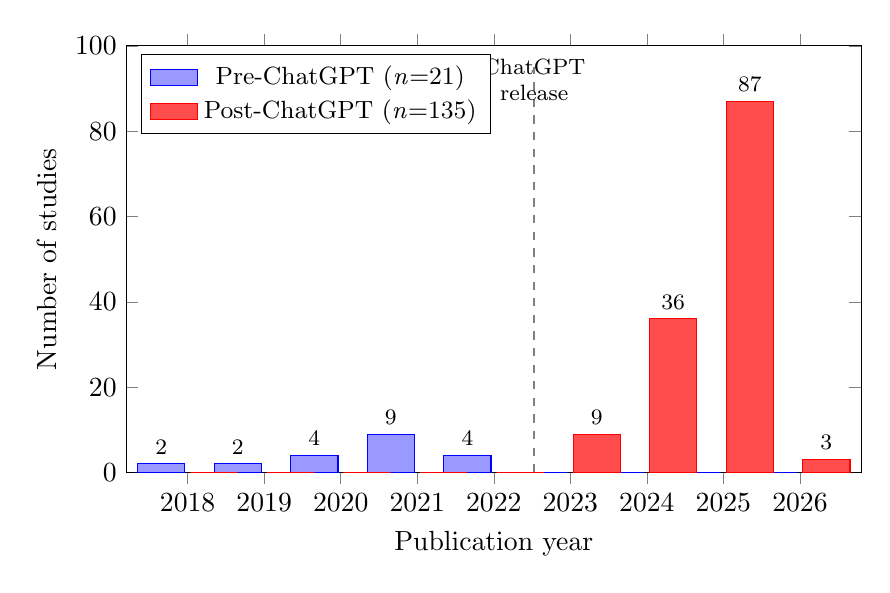
\begin{tikzpicture}
		\begin{axis}[
			ybar,
			width=0.9\textwidth,
			height=7cm,
			bar width=0.6cm,
			ylabel={Number of studies},
			xlabel={Publication year},
			symbolic x coords={2018, 2019, 2020, 2021, 2022, 2023, 2024, 2025, 2026},
			xtick=data,
			ymin=0,
			ymax=100,
			ytick={0, 20, 40, 60, 80, 100},
			nodes near coords,
			nodes near coords align={vertical},
			% Скрываем нулевые значения
			every node near coord/.append style={
				font=\footnotesize,
				/pgf/number format/assume math mode=true,
			},
			visualization depends on=\thisrow{show} \as \showmark,
			every node near coord/.append style={
				opacity=\showmark
			},
			legend style={at={(0.02,0.98)}, anchor=north west, font=\small},
			area legend,
			enlarge x limits=0.1,
			]
			
			% Pre-ChatGPT
			\addplot[fill=blue!40, draw=blue] table[meta=show] {
				x       y   show
				2018    2   1
				2019    2   1
				2020    4   1
				2021    9   1
				2022    4   1
				2023    0   0
				2024    0   0
				2025    0   0
				2026    0   0
			};
			
			% Post-ChatGPT
			\addplot[fill=red!70, draw=red] table[meta=show] {
				x       y   show
				2018    0   0
				2019    0   0
				2020    0   0
				2021    0   0
				2022    0   0
				2023    9   1
				2024    36  1
				2025    87  1
				2026    3   1
			};
			
			\legend{Pre-ChatGPT (\textit{n}=21), Post-ChatGPT (\textit{n}=135)}
			
			% Вертикальная линия между 2022 и 2023 (используем относительные координаты)
			\draw[dashed, thick, gray] (rel axis cs:0.555,0) -- (rel axis cs:0.555,0.95);
			\node[font=\footnotesize, align=center] at (rel axis cs:0.555,0.92) {ChatGPT\\release};
			
		\end{axis}
	\end{tikzpicture}
	\caption{Temporal distribution of included studies showing 6.4-fold increase post-ChatGPT.}
	\label{fig:temporal}
\end{figure}

Pre-ChatGPT studies (2017--2022) numbered only 21 (13.5\%), compared with 135 post-ChatGPT studies (86.5\%)~-- a 6.4-fold increase. The peak year was 2025, contributing 87 studies (55.8\%), indicating continued acceleration of research interest.

\subsubsection{Geographic distribution}

Figure~\ref{fig:geography} presents the geographic distribution of included studies based on first author institutional affiliation. Research is concentrated in East Asia, with China alone contributing nearly one-third of all studies.

\begin{figure}[htbp]
\centering
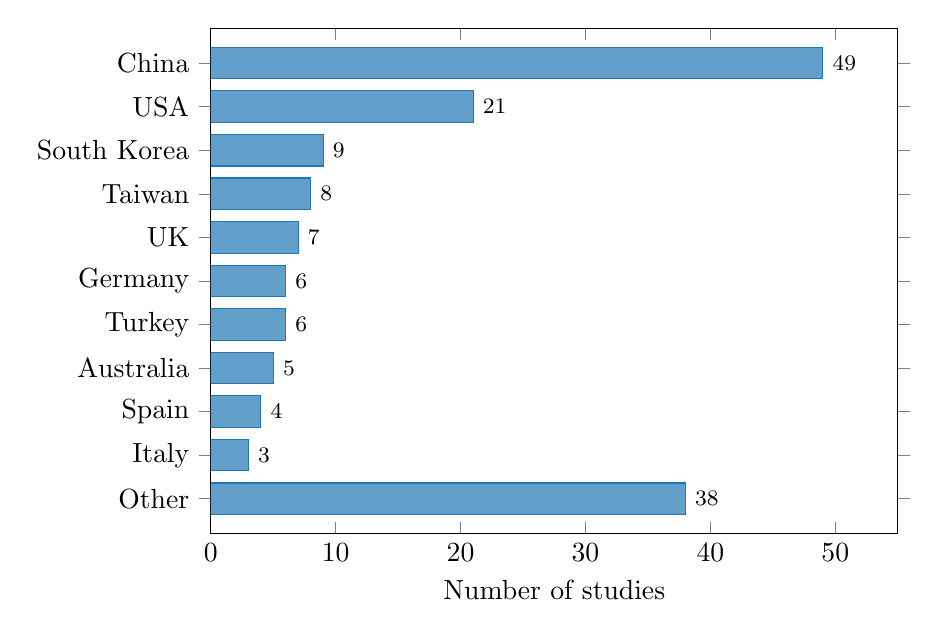
\begin{tikzpicture}
\begin{axis}[
    xbar,
    width=0.85\textwidth,
    height=8cm,
    bar width=0.4cm,
    xlabel={Number of studies},
    ylabel={},
    symbolic y coords={Other, Italy, Spain, Australia, Turkey, Germany, UK, Taiwan, South Korea, USA, China},
    ytick=data,
    xmin=0,
    xmax=55,
    nodes near coords,
    nodes near coords align={horizontal},
    every node near coord/.append style={font=\footnotesize},
    enlarge y limits=0.08,
]

\addplot[fill=primaryblue!70, draw=primaryblue] coordinates {
    (49,China)
    (21,USA)
    (9,South Korea)
    (8,Taiwan)
    (7,UK)
    (6,Germany)
    (6,Turkey)
    (5,Australia)
    (4,Spain)
    (3,Italy)
    (38,Other)
};

\end{axis}

%% Add regional annotations
%\node[font=\footnotesize, align=left] at (12.5, 5.8) {\textbf{East Asia: 42.3\%}};
%\node[font=\footnotesize, align=left] at (12.5, 3.5) {\textbf{Europe: 16.7\%}};
%\node[font=\footnotesize, align=left] at (12.5, 4.2) {\textbf{North America: 13.5\%}};

\end{tikzpicture}
\caption{Geographic distribution of included studies by first author affiliation.}
\label{fig:geography}
\end{figure}

East Asian countries (China, Taiwan, South Korea) collectively account for 42.3\% of the literature. Europe (including UK, Germany, Turkey, Spain, Italy) contributes 16.7\%, while North America (USA) contributes 13.5\%. Notable absences include Africa, Latin America, and most of South Asia, representing a significant geographic gap.

\subsubsection{Design discipline distribution}

Figure~\ref{fig:disciplines} presents the distribution across design disciplines. General design education dominates, with more specialized disciplines less well represented.

\begin{figure}[htbp]
\centering
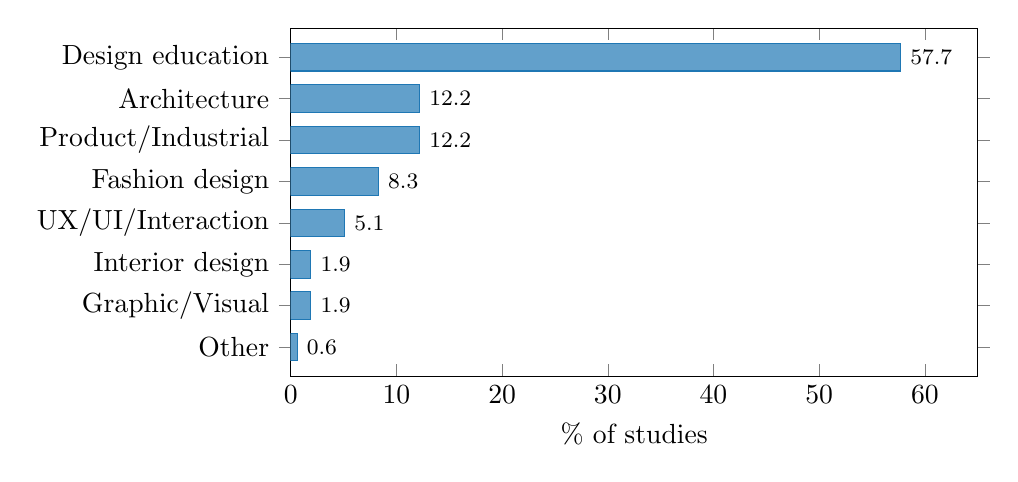
\begin{tikzpicture}
\begin{axis}[
    xbar,
    width=0.85\textwidth,
    height=6cm,
    bar width=0.35cm,
    xlabel={\% of studies},
    ylabel={},
    symbolic y coords={Other,Graphic/Visual,Interior design,UX/UI/Interaction,Fashion design,Product/Industrial,Architecture,Design education},
    ytick=data,
    xmin=0,
    xmax=65,
    nodes near coords,
    nodes near coords align={horizontal},
    every node near coord/.append style={font=\footnotesize},
    enlarge y limits=0.1,
]

\addplot[fill=primaryblue!70, draw=primaryblue] coordinates {
    (57.7,Design education)
    (12.2,Architecture)
    (12.2,Product/Industrial)
    (8.3,Fashion design)
    (5.1,UX/UI/Interaction)
    (1.9,Interior design)
    (1.9,Graphic/Visual)
    (0.6,Other)
};

\end{axis}
\end{tikzpicture}
\caption{Distribution of included studies by design discipline.}
\label{fig:disciplines}
\end{figure}

The dominance of general design education studies (57.7\%) reflects both the interdisciplinary nature of AI discussions and potential limitations in how studies characterize disciplinary focus. Architecture and product/industrial design are relatively well represented (12.2\% each), likely reflecting these disciplines' established engagement with computational tools. Critically, graphic/visual design (1.9\%) is dramatically underrepresented given the prominence of image generation AI tools~-- a significant gap discussed in section~\ref{sec:discussion}.

\subsubsection{Study design and methodological quality}

Table~\ref{tab:studydesign} categorizes included studies by methodological approach. Conceptual and framework papers constitute the largest category, reflecting the nascent state of empirical research.

\begin{table}[htbp]
\centering
\caption{Distribution of studies by study design and evidence quality.}
\label{tab:studydesign}
\small
\begin{tabular}{@{}lccc@{}}
\toprule
\hfill \textbf{Study design} & \textbf{\textit{n}} & \textbf{\%} & \textbf{Quality level} \\
\midrule
Conceptual/Framework & 36 & 23.1 & Lower \\
Experimental & 35 & 22.4 & Higher \\
Empirical (unspecified) & 31 & 19.9 & Lower \\
Review & 17 & 10.9 & Lower \\
Qualitative & 14 & 9.0 & Medium \\
Survey & 14 & 9.0 & Medium \\
Case study & 7 & 4.5 & Medium \\
Design-based research & 1 & 0.6 & Higher \\
Mixed methods & 1 & 0.6 & Higher \\
\midrule
\textbf{Total} & \textbf{156} & \textbf{100.0} & \\
\bottomrule
\end{tabular}
\end{table}

Categorizing by evidence quality: 37 studies (23.7\%) employed higher-quality designs (experimental, design-based research, mixed methods); 35 studies (22.4\%) used medium-quality designs (survey, qualitative, case study); and 84 studies (53.8\%) used lower-quality designs (conceptual, empirical without clear methodology, review). This distribution indicates limited empirical rigor in current literature.

\subsubsection{AI technology focus}

Table~\ref{tab:aitech} presents the distribution by AI technology type. Many studies reference AI in general terms rather than specifying particular technologies.

\begin{table}[htbp]
\centering
\caption{Distribution of studies by AI technology focus.}
\label{tab:aitech}
\small
\begin{tabular}{@{}lcc@{}}
\toprule
\hfill \textbf{AI technology category} & \textbf{\textit{n}} & \textbf{\%} \\
\midrule
AI (general) & 55 & 35.3 \\
Generative AI (general) & 29 & 18.6 \\
LLM/ChatGPT & 27 & 17.3 \\
Machine learning/Deep learning & 24 & 15.4 \\
LLM (unspecified) & 12 & 7.7 \\
Image generation AI & 9 & 5.8 \\
\midrule
\textbf{Total} & \textbf{156} & \textbf{100.0} \\
\bottomrule
\end{tabular}
\end{table}

Only 36 studies (23.1\%) mentioned specific AI tools by name. ChatGPT was most frequently mentioned (\textit{n}=23, 14.7\%), followed by Midjourney (\textit{n}=7, 4.5\%), Copilot (\textit{n}=6, 3.8\%), and GPT-4 (\textit{n}=4, 2.6\%). \citet{Turchi2023} provide one of few detailed analyses of how specific tools (DALL-E, MidJourney, StableDiffusion) impact creative processes, finding that ``interaction with LTGMs-based tools might impact creativity'' through feedback loops that shape user ideation.

\subsection{Thematic findings: pedagogical approaches (RQ2)}

\subsubsection{Pedagogical focus areas}

Figure~\ref{fig:pedagogy} presents the distribution of pedagogical focus areas. Studies could address multiple focus areas; percentages sum to more than 100\%.

\begin{figure}[htbp]
\centering
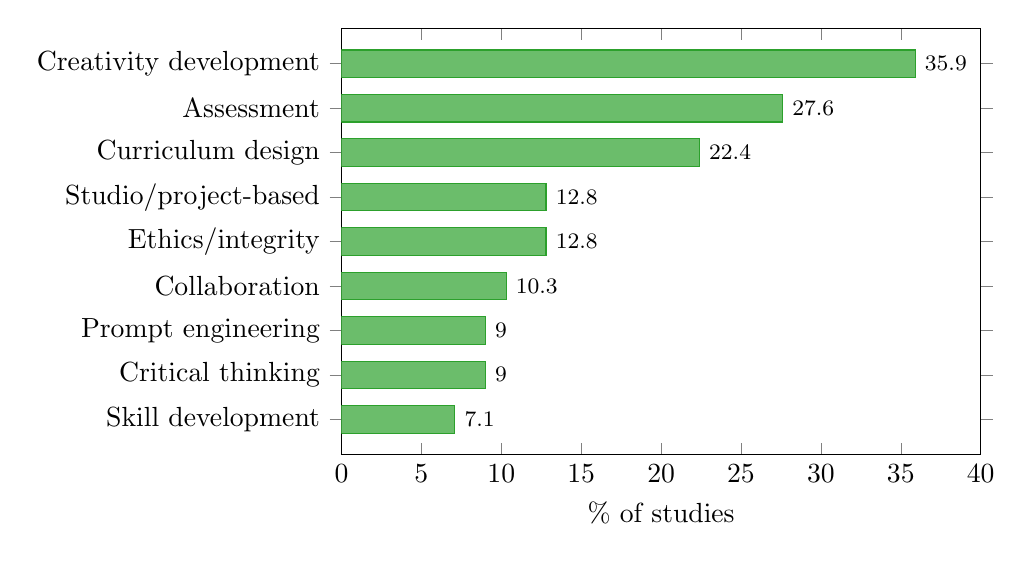
\begin{tikzpicture}
\begin{axis}[
    xbar,
    width=0.8\textwidth,
    height=7cm,
    bar width=0.35cm,
    xlabel={\% of studies},
    ylabel={},
    symbolic y coords={Skill development, Critical thinking, Prompt engineering, Collaboration, Ethics/integrity, Studio/project-based, Curriculum design, Assessment, Creativity development},
    ytick=data,
    xmin=0,
    xmax=40,
    nodes near coords,
    nodes near coords align={horizontal},
    every node near coord/.append style={font=\footnotesize},
    enlarge y limits=0.1,
]

\addplot[fill=tertiarygreen!70, draw=tertiarygreen] coordinates {
    (35.9,Creativity development)
    (27.6,Assessment)
    (22.4,Curriculum design)
    (12.8,Studio/project-based)
    (12.8,Ethics/integrity)
    (10.3,Collaboration)
    (9.0,Prompt engineering)
    (9.0,Critical thinking)
    (7.1,Skill development)
};

\end{axis}
\end{tikzpicture}
\caption{Distribution of pedagogical focus areas in included studies.}
\label{fig:pedagogy}
\end{figure}

Creativity development emerged as the dominant pedagogical concern (35.9\%), reflecting design education's core commitment to creative capability. \citet{MedelVera2025} found that GenAI can function ``as both a collaborator and provocateur in design pedagogy, facilitating creative ideation while inviting new pedagogical strategies centred on prompt literacy and reflective design''. Assessment implications (27.6\%) reflect widespread concern about evaluating work when AI assistance is readily available~-- \citet{Perkins2023} demonstrates that existing plagiarism detection tools ``are not yet equipped with methods to accurately detect AI-generated text''.

The emergence of prompt engineering as a pedagogical focus (9.0\%) suggests recognition of new competencies required in AI-mediated design work. \citet{Lee2024} developed an ``AI prompt guide'' for fashion design education, finding that students rated prompt guides 4.7 out of 5 for usefulness in generating creative design outputs through platforms like ChatGPT and Midjourney.

\subsubsection{Theoretical frameworks}

Only 41 studies (26.3\%) employed explicit theoretical frameworks. Table~\ref{tab:theory} presents the frameworks identified.

\begin{table}[htbp]
\centering
\caption{Theoretical frameworks employed in included studies.}
\label{tab:theory}
\small
\begin{tabular}{@{}lccl@{}}
\toprule
\hfill \textbf{Framework} & \textbf{\textit{n}} & \textbf{\%} & \hfill \textbf{Representative application} \\
\midrule
None specified & 115 & 73.7 & ~--  \\
Design thinking & 11 & 7.1 & Structuring AI-assisted ideation phases \\
Project-based learning & 8 & 5.1 & Integrating AI into studio projects \\
Experiential learning & 7 & 4.5 & Hands-on AI tool exploration \\
TPACK & 6 & 3.8 & Technology-pedagogy integration \\
UTAUT & 4 & 2.6 & Technology acceptance factors \\
Cognitive load theory & 3 & 1.9 & AI impact on mental effort \\
Constructivism & 3 & 1.9 & Student-centered AI learning \\
\bottomrule
\end{tabular}
\end{table}

The predominance of atheoretical work (73.7\%) represents a significant gap. Where theory was employed, the TPACK framework emerged as particularly relevant. \citet{Lee2024} applied TPACK to fashion design education, finding that AI integration ``enhances students' creativity and efficiency'' when technological, pedagogical, and content knowledge are systematically aligned. \citet{Boschman2015} demonstrate that teachers' TPACK develops through collaborative design activity, suggesting professional development pathways for AI integration.

\citet{Liu2025} employed both UTAUT (Unified Theory of Acceptance and Use of Technology) and AHP (Analytic Hierarchy Process) to evaluate generative AI tools in interior design education, finding that ``Stable Diffusion excelled in creativity, while Midjourney outperformed in aesthetics and functionality''. This comparative evaluation represents an emerging methodological approach for tool selection.

\subsection{Thematic findings: outcomes and challenges (RQ3)}

\subsubsection{Reported outcomes}

A striking finding is that 66.7\% of studies did not report specific measurable outcomes. Table~\ref{tab:outcomes} presents outcomes identified in remaining studies.

\begin{table}[htbp]
\centering
\caption{Reported outcomes in included studies.}
\label{tab:outcomes}
\small
\begin{tabular}{@{}lccl@{}}
\toprule
\hfill \textbf{Outcome category} & \textbf{\textit{n}} & \textbf{\%} & \hfill \textbf{Measurement approach} \\
\midrule
Not specified & 104 & 66.7 & ~--  \\
Learning outcomes & 30 & 19.2 & Pre-post tests, rubrics \\
Technology acceptance & 20 & 12.8 & Survey instruments (UTAUT) \\
Increased engagement & 6 & 3.8 & Self-report, observation \\
Enhanced creativity & 5 & 3.2 & CSI, expert evaluation \\
Improved efficiency & 1 & 0.6 & Time-on-task measures \\
\bottomrule
\end{tabular}
\end{table}

Among studies reporting outcomes, \citet{MedelVera2025} employed the Creativity Support Index (CSI) survey combined with semantic analysis and aesthetic evaluation, representing one of the more rigorous methodological approaches. Their findings indicate ``strong support for exploratory and goal-directed creativity, with high scores in exploration and results-worth-effort dimensions''. \citet{Dong2025} applied cognitive load theory and structural equation modeling, finding that ``AI-assisted paths significantly enhance design quality (72.43 vs.\ 65.60 in traditional paths)'' by reducing extraneous cognitive load while enhancing germane cognitive investment.

\subsubsection{Reported challenges}

Similarly, 74.4\% of studies did not document specific challenges. Table~\ref{tab:challenges} presents challenges identified.

\begin{table}[htbp]
\centering
\caption{Reported challenges in included studies.}
\label{tab:challenges}
\small
\begin{tabular}{@{}lccl@{}}
\toprule
\hfill \textbf{Challenge category} & \textbf{\textit{n}} & \textbf{\%} & \hfill \textbf{Nature of concern} \\
\midrule
Not specified & 116 & 74.4 & ~--  \\
Bias/fairness & 15 & 9.6 & Gender, ethnic representation \\
Implementation challenges & 10 & 6.4 & Technical, resource barriers \\
Faculty development needs & 6 & 3.8 & Training, support gaps \\
Academic integrity & 6 & 3.8 & Detection, attribution \\
Copyright/IP & 3 & 1.9 & Training data, ownership \\
Over-reliance/dependency & 2 & 1.3 & Skill atrophy concerns \\
\bottomrule
\end{tabular}
\end{table}

Bias concerns (9.6\%) emerged as the most documented challenge. \citet{Currie2024} conducted systematic evaluation of text-to-image AI bias, finding that ``60.6\% were male and 87.7\% were of a light skin tone'' across generated images, with DALL-E 3 including ``inherent biases associated with gender and ethnicity that demand more critical evaluation''. This has direct implications for design education contexts where representation matters.

Academic integrity concerns appeared in only 3.8\% of studies despite prominence in popular discourse. \citet{Perkins2023} provides comprehensive analysis, arguing that ``it is not the student use of any AI tools that defines whether plagiarism or a breach of academic integrity has occurred, but whether any use is made clear by the student''. \citet{Pudasaini2025} survey AI-generated plagiarism detection methods, concluding that existing tools ``struggle to accurately differentiate between human and AI essays''.

\subsection{Gap analysis (RQ4)}

The preceding analysis reveals six major gaps in current literature, visualized in figure~\ref{fig:gaps}:

\begin{figure}[htbp]
\centering
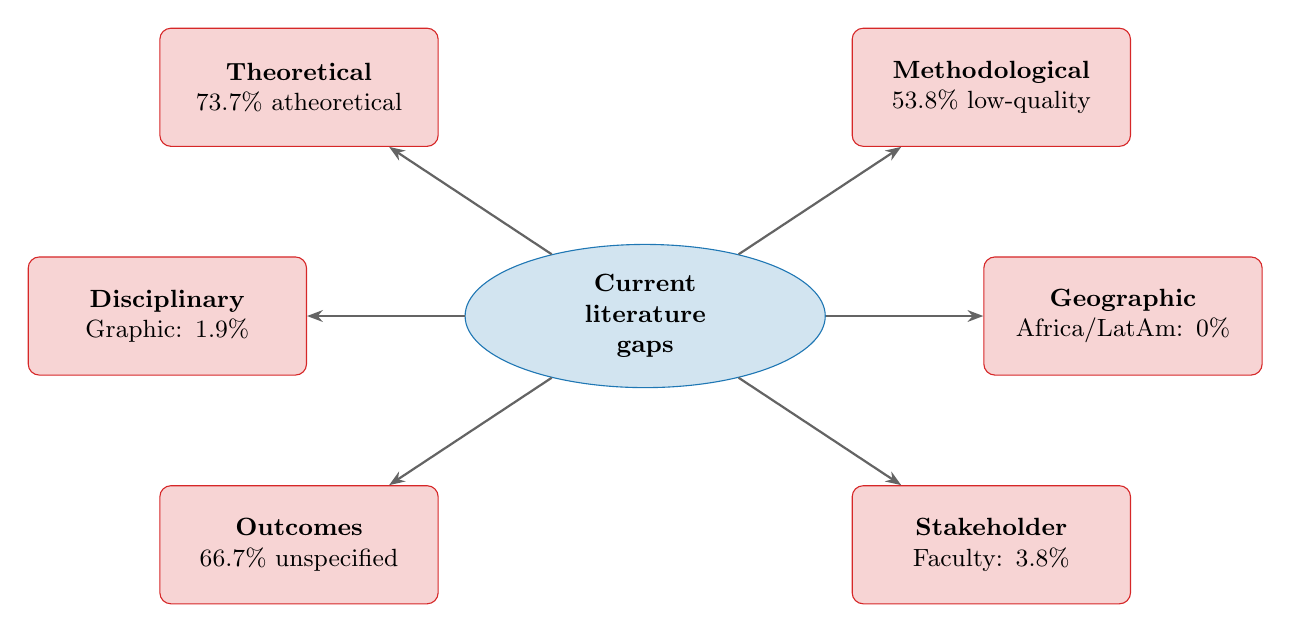
\begin{tikzpicture}[
    gap/.style={rectangle, draw=quaternaryred, fill=quaternaryred!20, text width=3.3cm, minimum height=1.5cm, align=center, font=\small, rounded corners},
    arrow/.style={-{Stealth[length=2mm]}, thick, darkgray}
]

% Central node
\node[ellipse, draw=primaryblue, fill=primaryblue!20, text width=3cm, align=center, font=\small\bfseries] (center) {Current\\literature\\gaps};

% Gap nodes
\node[gap, above left=1.5cm and 1cm of center] (g1) {\textbf{Theoretical}\\73.7\% atheoretical};
\node[gap, above right=1.5cm and 1cm of center] (g2) {\textbf{Methodological}\\53.8\% low-quality};
\node[gap, left=2cm of center] (g3) {\textbf{Disciplinary}\\Graphic: 1.9\%};
\node[gap, right=2cm of center] (g4) {\textbf{Geographic}\\Africa/LatAm: 0\%};
\node[gap, below left=1.5cm and 1cm of center] (g5) {\textbf{Outcomes}\\66.7\% unspecified};
\node[gap, below right=1.5cm and 1cm of center] (g6) {\textbf{Stakeholder}\\Faculty: 3.8\%};

% Arrows
\draw[arrow] (center) -- (g1);
\draw[arrow] (center) -- (g2);
\draw[arrow] (center) -- (g3);
\draw[arrow] (center) -- (g4);
\draw[arrow] (center) -- (g5);
\draw[arrow] (center) -- (g6);

\end{tikzpicture}
\caption{Six major gaps identified in current literature on AI in design education.}
\label{fig:gaps}
\end{figure}

\begin{enumerate}
	\item 
\textit{Theoretical gap.} With 73.7\% of studies lacking theoretical grounding, the field has limited capacity to explain \textit{why} observed phenomena occur or to build cumulative knowledge. The mechanisms by which AI affects learning, creativity, or design cognition remain underspecified.

	\item 
\textit{Methodological gap.} The predominance of conceptual papers (23.1\%) and lower-quality designs (53.8\%) limits strength of conclusions. No longitudinal studies were identified, precluding understanding of long-term effects. Only one mixed-methods study appeared.

	\item 
\textit{Disciplinary gap.} Graphic/visual design (1.9\%) is dramatically underrepresented given the relevance of image generation AI. Game design, service design, and textile/craft design are essentially absent despite AI tool applicability.

	\item 
\textit{Geographic gap.} The concentration in East Asia (42.3\%) and absence from Africa, Latin America, and most of South Asia limits generalizability and excludes important educational contexts.

	\item 
\textit{Outcomes gap.} With 66.7\% not specifying measurable outcomes, the evidence base for AI's educational effectiveness is thin. Studies reporting outcomes rarely use validated instruments or comparison conditions.

	\item 
\textit{Stakeholder gap.} Faculty perspectives (3.8\%) and student voices receive limited attention. Experiences, concerns, and strategies of primary participants in design education are underexplored.
\end{enumerate}

% ============================================================================
% 4. DISCUSSION
% ============================================================================

\section{Discussion}
\label{sec:discussion}

\subsection{Summary of evidence}

This scoping review identified and characterized \nstudies{} studies on AI in design education, revealing a field experiencing explosive growth~-- 6.4-fold increase post-ChatGPT~-- but facing significant gaps in theoretical grounding, methodological rigor, and empirical evidence. The literature concentrates in East Asia and North America, focuses predominantly on general design education rather than specific disciplines, and emphasizes creativity, assessment, and curriculum design as primary pedagogical concerns. While interest is intense, the evidence base for practice remains thin.

\subsection{The transformation of design learning}

The findings should be understood within broader context of design education's distinctive pedagogical traditions. Design education has long been characterized by what \citet{Schon1983} termed ``reflection-in-action''~-- the integration of thinking and doing that develops through sustained practice in studio settings. The signature pedagogies of design \cite{Shulman2005}~-- studio culture, design critique, iterative making~-- have historically served both to develop technical competencies and to socialize students into professional identity and values.

Generative AI disrupts this pedagogical model at multiple levels. If AI can produce design artifacts of professional quality, the relationship between practice and competence development requires reconceptualization. The focus on creativity development (35.9\% of studies) reflects design education's attempt to articulate what remains distinctively human in creative work. The attention to assessment (27.6\%) reflects the practical challenge of evaluating learning when traditional proxies~-- artifact quality~-- no longer reliably indicate individual capability.

\citet{Iranmanesh2024} frame this as a debate between views that ``text-to-image AI tools should be integrated into architectural education to prepare students for evolving professional practices'' versus concerns that ``an overreliance on AI poses a potential threat to the `learning-by-doing' pedagogy that is fundamental to design education''. This tension between innovation and tradition represents a fundamental challenge the field must navigate.

\subsection{From Maker to curator: reconceptualizing design identity}

A recurrent theme across the literature, though not always explicitly named, is the repositioning of the designer from maker to curator or orchestrator of AI-generated outputs. This transformation parallels earlier technological transitions~-- from craftsperson to CAD operator, from drafter to parametric designer~-- but with a crucial difference: generative AI intervenes not merely in execution but in ideation itself.

\citet{Sennett2008} argued that craftsmanship~-- sustained practice of making things well~-- develops not only skill but also character, patience, and judgment. The educational question is whether curating AI outputs can develop equivalent capacities, or whether something essential is lost when the hand no longer guides the making. The limited attention to this question in current literature (skill development appears in only 7.1\% of studies) represents a significant conceptual gap.

\citet{MedelVera2025} offer one productive framing, finding that GenAI can function as ``both a collaborator and provocateur in design pedagogy''. Their emphasis on ``prompt literacy and reflective design'' suggests that new forms of design thinking may emerge from human-AI collaboration rather than being simply diminished versions of traditional practice. Similarly, \citet{Dong2025} demonstrate that AI assistance can reduce extraneous cognitive load while enhancing ``deep, innovative thinking''~-- suggesting that thoughtful integration might actually enhance rather than undermine educational outcomes.

\subsection{Theoretical underdevelopment and pathways forward}

The finding that 73.7\% of studies lack theoretical frameworks is perhaps the most consequential gap identified. Without theory, research produces observations without explanations, accumulates facts without building understanding. The field lacks shared language for discussing AI's effects on design cognition, design learning, or design identity.

Several theoretical traditions could potentially inform this work:

\begin{itemize}
	\item 
\textit{TPACK (Technological Pedagogical Content Knowledge):} The 3.8\% of studies employing TPACK demonstrate its relevance \cite{Lee2024, Bower2017}. This framework's emphasis on the intersection of technological, pedagogical, and content knowledge maps directly onto the challenge of integrating AI tools into design curricula. \citet{Polly2020} argue that Vygotsky's zone of proximal development can inform TPACK development, suggesting developmental pathways for AI integration competencies.

	\item 
\textit{Cognitive load theory:} \citet{Dong2025} demonstrate how this framework illuminates AI's educational effects, finding that AI reduces extraneous load while potentially supporting germane cognitive investment. This suggests a research program examining how different AI integrations affect the cognitive demands of design learning.

	\item 
\textit{Reflective practice:} \citet{Schon1983} remains foundational for understanding design learning. How reflection-in-action functions when the ``action'' is prompting AI systems rather than physically making artifacts deserves sustained theoretical attention.

	\item 
\textit{Creativity support frameworks:} \citet{MedelVera2025} employ the Creativity Support Index, demonstrating how established creativity research methods can be applied to AI contexts. Systematic application of creativity theories could ground claims about AI's impact on creative development.
\end{itemize}

\subsection{Pedagogical implications}

\subsubsection{Curriculum design}

The emergence of prompt engineering as a pedagogical focus (9.0\%) indicates recognition of new competencies, but systematic frameworks for sequencing AI skill development remain absent. Drawing on findings, curricula may need to address:

\begin{itemize}%[leftmargin=1cm, itemsep=0.2em]
    \item \textit{AI literacy} -- critical understanding of how AI systems work, their capabilities, limitations, and societal implications \cite{Pudasaini2025};
    \item \textit{prompt craft} -- iterative, reflective practice of formulating effective prompts~-- arguably a new form of design thinking \cite{Lee2024};
    \item \textit{curation and judgment} -- capacity to evaluate, select, and refine AI outputs according to design criteria \cite{MedelVera2025};
    \item \textit{human-AI collaboration} -- strategies for integrating AI into personal creative workflows while maintaining authorial voice \cite{Turchi2023};
    \item \textit{ethical reasoning} -- frameworks for making decisions about when and how AI use is appropriate \cite{Buragohain2025}.
\end{itemize}

\subsubsection{Assessment reform}

The prominence of assessment concerns (27.6\%) reflects genuine difficulty evaluating learning when AI assistance is ubiquitous. \citet{Perkins2023} demonstrates that existing detection tools cannot reliably identify AI-generated content. \citet{Deluca2025} propose the ``AI3 Model'' integrating AI considerations with academic integrity and assessment innovation.

Traditional assessment methods focusing on final artifacts may need supplementation with process documentation revealing human contribution, oral examinations probing understanding and decision-making, in-class exercises establishing baseline capabilities, portfolio curation emphasizing selection and reflection over production, and peer critique skills demonstrating ability to evaluate design quality.

\subsubsection{Faculty development}

Faculty development needs appear in only 3.8\% of studies~-- striking underrepresentation given that educators implement pedagogical change. \citet{Fleischmann2024} found students using generative AI ``in an ad hoc way'' with ``sceptical view of its creative output'', suggesting faculty guidance is needed but often absent. Effective AI integration requires that faculty develop their own competencies, reconceptualize their roles from knowledge transmitters to learning facilitators, redesign assignments and assessments, navigate ethical complexities without clear institutional guidance, and model appropriate AI use for students.

\subsection{Limitations}
\label{sec:limitations}

This review has several limitations that inform interpretation of findings. The search was restricted to Web of Science Core Collection, meaning relevant literature may exist in other databases such as Scopus, and ERIC, as well as in design-specific repositories or gray literature. This decision prioritized depth over breadth.

Screening and data extraction were conducted by a single reviewer, introducing potential for bias and error. While consistent criteria application was attempted, dual independent screening would have been preferable. Additionally, full-text assessment relied primarily on abstract content due to access constraints, meaning some studies may have been misclassified based on limited information.

The English language requirement excluded potentially relevant research published in other languages, a limitation of particular concern given the concentration of research activity in China and South Korea. The field also evolves rapidly, meaning publications after the search date are not captured and the landscape may have shifted since data collection.

Finally, included studies vary widely in design, context, and focus, limiting the depth of synthesis possible. This heterogeneity reflects the field's emerging state but complicates drawing definitive conclusions about the current state of knowledge.

\subsection{Future research directions}

The gaps identified suggest a structured research agenda:

\begin{enumerate}[label={Priority}~\arabic*:,leftmargin=*]
	\item 

\textit{Longitudinal studies.} The absence of longitudinal research precludes understanding how AI integration affects learning over time. Studies tracking student cohorts through design programs, documenting skill development, creative evolution, and professional preparation, are urgently needed.

	\item 

\textit{Theoretically grounded empirical research.} Studies should explicitly test theoretical propositions about mechanisms and moderators. Does AI assistance reduce cognitive load, freeing capacity for higher-order thinking, or short-circuit productive struggle through which learning occurs? Under what conditions does AI enhance versus diminish creativity?

	\item 

\textit{Discipline-specific studies.} Graphic design, game design, and other underrepresented disciplines require focused investigation. The applicability and implications of AI tools likely vary across design domains in ways current literature cannot illuminate.

	\item 

\textit{Stakeholder research.} Studies centering faculty and student experiences, using qualitative and mixed methods, are needed to complement predominantly conceptual literature. Understanding how educators actually navigate this transition, and how students integrate AI into learning, is essential.

	\item 

\textit{Assessment development.} Research developing and validating assessment approaches for AI-mediated design education is urgently needed, including both instruments for measuring learning outcomes and frameworks for evaluating AI-assisted work.

	\item 

\textit{Ethical and policy research.} Studies examining academic integrity practices, attribution norms, equity implications, and institutional policy responses would address underexplored areas. \citet{Mazzi2024} explores authorship in AI-generated works, representing an emerging research direction.
\end{enumerate}

% ============================================================================
% 5. CONCLUSION
% ============================================================================

\section{Conclusion}
\label{sec:conclusion}

This scoping review has mapped the emerging research landscape on generative AI in design education, identifying \nstudies{} studies published between 2017 and 2026. The findings reveal a field experiencing explosive growth but facing significant challenges. The 6.4-fold increase in publications following ChatGPT's release demonstrates intense scholarly interest; the gaps in theoretical grounding (73.7\% atheoretical), outcome reporting (66.7\% unspecified), and methodological rigor (53.8\% lower-quality designs) demonstrate the distance yet to travel.

The title of this paper~-- \textit{From maker to curator}~-- captures a transformation the literature addresses implicitly but rarely names directly. As AI systems assume capacities historically cultivated through design education, the fundamental question becomes: what should design education develop now? The studies reviewed suggest emerging answers~-- creativity, judgment, ethics, critical AI literacy, prompt craft~-- but empirical evidence for how best to develop these capacities remains thin.

For design educators, this review offers both validation and challenge. Validation: the concerns navigated daily~-- about creativity, assessment, integrity, identity~-- are shared across the global design education community. Challenge: the evidence base for practice remains limited, and educators are largely navigating without maps.

For researchers, this review provides orientation and direction. The gaps identified~-- theoretical, methodological, disciplinary, geographic~-- are not merely academic; they represent urgent needs for knowledge that can inform practice. The research agenda proposed offers concrete priorities for contributing to this rapidly evolving field.

For institutional leaders and policymakers, the review underscores need for investment in faculty development, assessment infrastructure, and ethical frameworks. The transformation underway is not a temporary disruption to be weathered but a fundamental shift requiring strategic response.

The future of design education in the age of AI remains unwritten. This review has attempted to map what is known~-- and what is not yet known~-- as the design education community writes that future together. In this new paradigm, as contemporary practitioners observe, ``the value of the designer is no longer found in the ability to draw or code but in the ability to think, judge, and curate''. The choices made in the coming years will shape not only what designers know how to do, but who they understand themselves to be.

% ============================================================================
% DECLARATIONS
% ============================================================================

%\section*{Declarations}
%
%\textbf{Author Contributions:} [Author] conceived the study, conducted the search and screening, extracted and analyzed data, and wrote the manuscript.

\begin{funding}
	This research received no external funding.
\end{funding}

%\textbf{Funding:} [No funding received / funding statement to be completed]

%\textbf{Conflicts of Interest:} The author declares no conflicts of interest.

%\textbf{Data Availability:} The complete data extraction table is available as supplementary material. The list of included studies is available upon reasonable request.

%\textbf{Ethics Approval:} Not applicable. This study involved secondary analysis of published literature and did not involve human participants.

% ============================================================================
% ACKNOWLEDGMENTS
% ============================================================================

%\section*{Acknowledgments}
%
%[Placeholder for acknowledgments]

% ============================================================================
% REFERENCES
% ============================================================================

%\newpage
\bibliography{references}

\appendix
% ============================================================================
% APPENDICES
% ============================================================================

%\newpage
%\begin{appendices}

\section{PRISMA-ScR checklist}
\label{app:prisma}

\small
\begin{longtable}{@{}lll@{}}
\toprule
\hfill\textbf{PRISMA-ScR item} & \hfill\textbf{Location} & \hfill\textbf{Notes} \\
\midrule
\endfirsthead
\midrule
\hfil \textbf{PRISMA-ScR item} & \textbf{Location} & \textbf{Notes} \\
\midrule
\endhead
\bottomrule
\endfoot
Title & Title & Identifies as scoping review \\
Structured summary & Abstract & All required elements present \\
Rationale & Section 1.4 & Need for synthesis established \\
Objectives & Section 1.5 & Four RQs explicitly stated \\
Protocol registration & Section 2.1 & Not registered; noted \\
Eligibility criteria & Section 2.2 & Tables 1--2; PCC framework \\
Information sources & Section 2.3 & Web of Science described \\
Search strategy & Section 2.4 & Complete strings provided \\
Selection process & Section 2.5 & Two-stage screening \\
Data charting & Section 2.6 & 21 variables described \\
Data items & Section 2.6 & Variables listed by domain \\
Critical appraisal & Section 2.6 & N/A for scoping review \\
Synthesis methods & Section 2.7 & Descriptive + thematic \\
Selection of sources & Section 3.1 & Figure 1; PRISMA flow \\
Characteristics & Section 3.2 & Tables 3--6; figures 2--5 \\
Results of sources & Section 3.3 & Organized by theme \\
Synthesis of results & Section 3.4 & Gap analysis integrated \\
Limitations & Section 4.6 & Six limitations discussed \\
Conclusions & Section 5 & Summary and implications \\
Funding & Declarations & Statement provided \\
\end{longtable}

%\end{appendices}

\end{document}
